% \newpage
\afterpage{%
    % \newpage
    \clearpage
%     \thispagestyle{empty}
    
%         \AddToShipoutPictureBG*{%
%   \AtPageLowerLeft{%
%     \raisebox{\dimexpr.5\paperheight-.5\height}{%
%       \makebox[.1\paperwidth][r]{%
%         \rotatebox{90}{\thepage}
%       }% \makebox
%     }% \raisebox
%   }% \AtPageCenter
% }% \AddToShipoutPictureBG*

        \begin{landscape}% Landscape page
        % \centering

        \begin{table}[]
        \hspace{-\marginparsep}    
        \hspace{-0.5\marginparwidth}
        \resizebox{1.65\textwidth}{!}{%
        \begin{tabular}{l|ccccccccc|l}
        \cline{2-10}
         & \multicolumn{9}{c|}{Observations per Baseline} &  \\ \hline
        \multicolumn{1}{|l|}{Baseline} & \multicolumn{1}{c|}{\begin{tabular}[c]{@{}c@{}}Own \\ Information\end{tabular}} & \multicolumn{1}{c|}{\begin{tabular}[c]{@{}c@{}}Octree \\ Observations\end{tabular}} & \multicolumn{1}{c|}{\begin{tabular}[c]{@{}c@{}}Vision \\ of Voxels\end{tabular}} & \multicolumn{1}{c|}{\begin{tabular}[c]{@{}c@{}}Pigeon \\ Observations\end{tabular}} & \multicolumn{1}{l|}{\begin{tabular}[c]{@{}l@{}}Speed Sensitivity \\ to Targets in FOV\end{tabular}} & \multicolumn{1}{c|}{\begin{tabular}[c]{@{}c@{}}Shortest Path\\  Observations\end{tabular}} & \multicolumn{1}{c|}{\begin{tabular}[c]{@{}c@{}}Detector \\ Observations\end{tabular}} & \multicolumn{1}{c|}{\begin{tabular}[c]{@{}c@{}}Semantic Curiosity \\ Observations\end{tabular}} & \begin{tabular}[c]{@{}c@{}}Semantic Entropy \\ Observations\end{tabular} & \multicolumn{1}{l|}{Comment} \\ \hline
        \multicolumn{1}{|l|}{Random Walk} & \multicolumn{1}{c|}{✔️} & \multicolumn{1}{c|}{} & \multicolumn{1}{c|}{} & \multicolumn{1}{c|}{} & \multicolumn{1}{c|}{} & \multicolumn{1}{c|}{} & \multicolumn{1}{c|}{} & \multicolumn{1}{c|}{} &  & \multicolumn{1}{l|}{Simple agent that observes its speed and position in 3D space.} \\ \hline
        \multicolumn{1}{|l|}{Octree Agent} & \multicolumn{1}{c|}{✔️} & \multicolumn{1}{c|}{✔️} & \multicolumn{1}{c|}{} & \multicolumn{1}{c|}{✔️} & \multicolumn{1}{c|}{} & \multicolumn{1}{c|}{} & \multicolumn{1}{c|}{} & \multicolumn{1}{c|}{} &  & \multicolumn{1}{l|}{Derived* agent that can observe the amount of octree nodes it discovers on timestep t.} \\ \hline
        \multicolumn{1}{|l|}{Voxel (R\_VOX norm)} & \multicolumn{1}{c|}{✔️} & \multicolumn{1}{c|}{} & \multicolumn{1}{c|}{✔️} & \multicolumn{1}{c|}{} & \multicolumn{1}{c|}{✔️} & \multicolumn{1}{c|}{} & \multicolumn{1}{c|}{} & \multicolumn{1}{c|}{} &  & \multicolumn{1}{l|}{Derived* agent that can observe the voxels in the environment. Voxels reward is normalized.} \\ \hline
        \multicolumn{1}{|l|}{Voxel (R\_VOX str: 0.25)} & \multicolumn{1}{c|}{✔️} & \multicolumn{1}{c|}{} & \multicolumn{1}{c|}{✔️} & \multicolumn{1}{c|}{} & \multicolumn{1}{c|}{✔️} & \multicolumn{1}{c|}{} & \multicolumn{1}{c|}{} & \multicolumn{1}{c|}{} &  & \multicolumn{1}{l|}{Derived* agent that can observe the voxels in the environment. Voxel reward strength is set to 25\%} \\ \hline
        \multicolumn{1}{|l|}{Voxel (R\_VOX str: 0.50)} & \multicolumn{1}{c|}{✔️} & \multicolumn{1}{c|}{} & \multicolumn{1}{c|}{✔️} & \multicolumn{1}{c|}{} & \multicolumn{1}{c|}{✔️} & \multicolumn{1}{c|}{} & \multicolumn{1}{c|}{} & \multicolumn{1}{c|}{} &  & \multicolumn{1}{l|}{Derived* agent that can observe the voxels in the environment. Voxel reward strength is set to 50\%} \\ \hline
        \multicolumn{1}{|l|}{Voxel (R\_VOX str: 0.75)} & \multicolumn{1}{c|}{✔️} & \multicolumn{1}{c|}{} & \multicolumn{1}{c|}{✔️} & \multicolumn{1}{c|}{} & \multicolumn{1}{c|}{✔️} & \multicolumn{1}{c|}{} & \multicolumn{1}{c|}{} & \multicolumn{1}{c|}{} &  & \multicolumn{1}{l|}{Derived* agent that can observe the voxels in the environment. Voxel reward strength is set to 75\%} \\ \hline
        \multicolumn{1}{|l|}{Voxel (R\_VOX str: 1.00)} & \multicolumn{1}{c|}{✔️} & \multicolumn{1}{c|}{} & \multicolumn{1}{c|}{✔️} & \multicolumn{1}{c|}{} & \multicolumn{1}{c|}{✔️} & \multicolumn{1}{c|}{} & \multicolumn{1}{c|}{} & \multicolumn{1}{c|}{} &  & \multicolumn{1}{l|}{Derived* agent that can observe the voxels in the environment. Voxel reward strength is set to 100\%} \\ \hline
        \multicolumn{1}{|l|}{Shortest Path + Vision} & \multicolumn{1}{c|}{✔️} & \multicolumn{1}{c|}{} & \multicolumn{1}{c|}{✔️} & \multicolumn{1}{c|}{} & \multicolumn{1}{c|}{✔️} & \multicolumn{1}{c|}{} & \multicolumn{1}{c|}{} & \multicolumn{1}{c|}{} &  & \multicolumn{1}{l|}{Derived* agent that has more information about where the target is in 3D space and can observe voxels.} \\ \hline
        \multicolumn{1}{|l|}{Shortest Path} & \multicolumn{1}{c|}{✔️} & \multicolumn{1}{c|}{} & \multicolumn{1}{c|}{} & \multicolumn{1}{c|}{} & \multicolumn{1}{c|}{✔️} & \multicolumn{1}{c|}{✔️} & \multicolumn{1}{c|}{} & \multicolumn{1}{c|}{} &  & \multicolumn{1}{l|}{Derived* agent that has more information about where the target is in 3D space.} \\ \hline
        \multicolumn{1}{|l|}{Object Detection + pure} & \multicolumn{1}{c|}{✔️} & \multicolumn{1}{c|}{} & \multicolumn{1}{c|}{} & \multicolumn{1}{c|}{} & \multicolumn{1}{c|}{✔️} & \multicolumn{1}{c|}{} & \multicolumn{1}{c|}{} & \multicolumn{1}{c|}{} &  & \multicolumn{1}{l|}{Simple agent that observes the output from the object detector.} \\ \hline
        \multicolumn{1}{|l|}{Object Detection} & \multicolumn{1}{c|}{✔️} & \multicolumn{1}{c|}{} & \multicolumn{1}{c|}{} & \multicolumn{1}{c|}{} & \multicolumn{1}{c|}{✔️} & \multicolumn{1}{c|}{} & \multicolumn{1}{c|}{✔️} & \multicolumn{1}{c|}{} &  & \multicolumn{1}{l|}{Derived* agent that observes the output from the object detector.} \\ \hline
        \multicolumn{1}{|l|}{Semantic Curiosity} & \multicolumn{1}{c|}{✔️} & \multicolumn{1}{c|}{} & \multicolumn{1}{c|}{} & \multicolumn{1}{c|}{} & \multicolumn{1}{c|}{✔️} & \multicolumn{1}{c|}{} & \multicolumn{1}{c|}{} & \multicolumn{1}{c|}{✔️} &  & \multicolumn{1}{l|}{Derived* agent that observes the rationalized class density present in the environment each timestep t.} \\ \hline
        \multicolumn{1}{|l|}{Ultron (Semantic Entropy)} & \multicolumn{1}{c|}{✔️} & \multicolumn{1}{c|}{} & \multicolumn{1}{c|}{} & \multicolumn{1}{c|}{} & \multicolumn{1}{c|}{✔️} & \multicolumn{1}{c|}{} & \multicolumn{1}{c|}{} & \multicolumn{1}{c|}{} &  & \multicolumn{1}{l|}{Derived* agent that observes the lingering penalty strength present in the environment each timestep t. Voxel reward is normalized.} \\ \hline
        \multicolumn{1}{|l|}{Ultron (R\_VOX str: 0.5)} & \multicolumn{1}{c|}{✔️} & \multicolumn{1}{c|}{✔️} & \multicolumn{1}{c|}{✔️} & \multicolumn{1}{c|}{✔️} & \multicolumn{1}{c|}{✔️} & \multicolumn{1}{c|}{} & \multicolumn{1}{c|}{} & \multicolumn{1}{c|}{} & ✔️ & \multicolumn{1}{l|}{Derived* agent as above. Voxel reward strength is set to 50\%} \\ \hline
        \multicolumn{1}{|l|}{Ultron (R\_VOX str: 1.0)} & \multicolumn{1}{c|}{✔️} & \multicolumn{1}{c|}{✔️} & \multicolumn{1}{c|}{✔️} & \multicolumn{1}{c|}{✔️} & \multicolumn{1}{c|}{✔️} & \multicolumn{1}{c|}{} & \multicolumn{1}{c|}{} & \multicolumn{1}{c|}{} & ✔️ & \multicolumn{1}{l|}{Derived* agent as above. Voxel reward strength is set to 100\%} \\ \hline
        \end{tabular}%
        }
        \caption{Diverse agent behavior variants and the observations they receive.}
        \label{appendix:baselines_observations}
        \end{table}
        
            % \usepackage{graphicx}
       
        \begin{table}[]
        \hspace{-\marginparsep}    
        \hspace{-0.5\marginparwidth}
        \resizebox{1.65\textwidth}{!}{%
            \begin{tabular}{l|cccccccc|l}
            \cline{2-9}
             & \multicolumn{8}{c|}{Rewards per Baseline} &  \\ \hline
            \multicolumn{1}{|l|}{Baseline} & \multicolumn{1}{c|}{\begin{tabular}[c]{@{}c@{}}Train Moving \\ Forward\end{tabular}} & \multicolumn{1}{c|}{\begin{tabular}[c]{@{}c@{}}Train \\ Speed\end{tabular}} & \multicolumn{1}{c|}{\begin{tabular}[c]{@{}c@{}}Train Octree \\ Nodes Discovery\end{tabular}} & \multicolumn{1}{c|}{\begin{tabular}[c]{@{}c@{}}Train Voxel \\ Discovery\end{tabular}} & \multicolumn{1}{c|}{\begin{tabular}[c]{@{}c@{}}Train Shortest \\ Path\end{tabular}} & \multicolumn{1}{c|}{\begin{tabular}[c]{@{}c@{}}Train Object \\ Detection\end{tabular}} & \multicolumn{1}{c|}{\begin{tabular}[c]{@{}c@{}}Train Semantic \\ Curiosity\end{tabular}} & \begin{tabular}[c]{@{}c@{}}Train Semantic \\ Entropy\end{tabular} & \multicolumn{1}{l|}{Comment} \\ \hline
            \multicolumn{1}{|l|}{Random Walk} & \multicolumn{1}{c|}{✔️} & \multicolumn{1}{c|}{✔️} & \multicolumn{1}{c|}{} & \multicolumn{1}{c|}{} & \multicolumn{1}{c|}{} & \multicolumn{1}{c|}{} & \multicolumn{1}{c|}{} &  & \multicolumn{1}{l|}{Simple agent that learns to move to reach a minimum target speed.} \\ \hline
            \multicolumn{1}{|l|}{Octree Agent} & \multicolumn{1}{c|}{✔️} & \multicolumn{1}{c|}{✔️} & \multicolumn{1}{c|}{✔️} & \multicolumn{1}{c|}{} & \multicolumn{1}{c|}{} & \multicolumn{1}{c|}{} & \multicolumn{1}{c|}{} &  & \multicolumn{1}{l|}{Derived* agent that learns how to discover octree nodes while it moves.} \\ \hline
            \multicolumn{1}{|l|}{Voxel (R\_VOX norm)} & \multicolumn{1}{c|}{✔️} & \multicolumn{1}{c|}{✔️} & \multicolumn{1}{c|}{} & \multicolumn{1}{c|}{✔️} & \multicolumn{1}{c|}{} & \multicolumn{1}{c|}{} & \multicolumn{1}{c|}{} &  & \multicolumn{1}{l|}{""                                                                                             ""} \\ \hline
            \multicolumn{1}{|l|}{Voxel (R\_VOX str: 0.25)} & \multicolumn{1}{c|}{✔️} & \multicolumn{1}{c|}{✔️} & \multicolumn{1}{c|}{} & \multicolumn{1}{c|}{✔️} & \multicolumn{1}{c|}{} & \multicolumn{1}{c|}{} & \multicolumn{1}{c|}{} &  & \multicolumn{1}{l|}{""                                                                                             ""} \\ \hline
            \multicolumn{1}{|l|}{Voxel (R\_VOX str: 0.50)} & \multicolumn{1}{c|}{✔️} & \multicolumn{1}{c|}{✔️} & \multicolumn{1}{c|}{} & \multicolumn{1}{c|}{✔️} & \multicolumn{1}{c|}{} & \multicolumn{1}{c|}{} & \multicolumn{1}{c|}{} &  & \multicolumn{1}{l|}{""                                                                                             ""} \\ \hline
            \multicolumn{1}{|l|}{Voxel (R\_VOX str: 0.75)} & \multicolumn{1}{c|}{✔️} & \multicolumn{1}{c|}{✔️} & \multicolumn{1}{c|}{} & \multicolumn{1}{c|}{✔️} & \multicolumn{1}{c|}{} & \multicolumn{1}{c|}{} & \multicolumn{1}{c|}{} &  & \multicolumn{1}{l|}{""                                                                                             ""} \\ \hline
            \multicolumn{1}{|l|}{Voxel (R\_VOX str: 1.00)} & \multicolumn{1}{c|}{✔️} & \multicolumn{1}{c|}{✔️} & \multicolumn{1}{c|}{} & \multicolumn{1}{c|}{✔️} & \multicolumn{1}{c|}{} & \multicolumn{1}{c|}{} & \multicolumn{1}{c|}{} &  & \multicolumn{1}{l|}{""                                                                                             ""} \\ \hline
            \multicolumn{1}{|l|}{Shortest Path + Vision} & \multicolumn{1}{c|}{✔️} & \multicolumn{1}{c|}{✔️} & \multicolumn{1}{c|}{} & \multicolumn{1}{c|}{✔️} & \multicolumn{1}{c|}{✔️} & \multicolumn{1}{c|}{} & \multicolumn{1}{c|}{} &  & \multicolumn{1}{l|}{Derived* agent that learns to move directly to the next target. Found voxels provide a normalized reward.} \\ \hline
            \multicolumn{1}{|l|}{Shortest Path} & \multicolumn{1}{c|}{✔️} & \multicolumn{1}{c|}{✔️} & \multicolumn{1}{c|}{} & \multicolumn{1}{c|}{✔️} & \multicolumn{1}{c|}{✔️} & \multicolumn{1}{c|}{} & \multicolumn{1}{c|}{} &  & \multicolumn{1}{l|}{Derived* agent that learns to move directly to the next target. Found voxels provide a normalized reward.} \\ \hline
            \multicolumn{1}{|l|}{Object Detection + pure} & \multicolumn{1}{c|}{✔️} & \multicolumn{1}{c|}{} & \multicolumn{1}{c|}{} & \multicolumn{1}{c|}{✔️} & \multicolumn{1}{c|}{} & \multicolumn{1}{c|}{✔️} & \multicolumn{1}{c|}{} &  & \multicolumn{1}{l|}{Derived* agent that learns how to maximize object detections. Found voxels provide a normalized reward.} \\ \hline
            \multicolumn{1}{|l|}{Object Detection} & \multicolumn{1}{c|}{✔️} & \multicolumn{1}{c|}{✔️} & \multicolumn{1}{c|}{} & \multicolumn{1}{c|}{✔️} & \multicolumn{1}{c|}{} & \multicolumn{1}{c|}{✔️} & \multicolumn{1}{c|}{} &  & \multicolumn{1}{l|}{Derived* agent that learns how to maximize object detections. Found voxels provide a normalized reward.} \\ \hline
            % \multicolumn{1}{|l|}{Semantic Curiosity} & \multicolumn{1}{c|}{✔️} & \multicolumn{1}{c|}{✔️} & \multicolumn{1}{c|}{} & \multicolumn{1}{c|}{✔️} & \multicolumn{1}{c|}{} & \multicolumn{1}{c|}{} & \multicolumn{1}{c|}{✔️} &  & \multicolumn{1}{l|}{Derived* agent that learns how to maximize the temporal class density.} \\ \hline
            % \multicolumn{1}{|l|}{Ultron (Semantic Entropy)} & \multicolumn{1}{c|}{✔️} & \multicolumn{1}{c|}{✔️} & \multicolumn{1}{c|}{} & \multicolumn{1}{c|}{✔️} & \multicolumn{1}{c|}{} & \multicolumn{1}{c|}{} & \multicolumn{1}{c|}{} & ✔️ & \multicolumn{1}{l|}{Derived* agent that learns how to discover octree nodes and scan voxels. Benefits from a lingering penalty strength regulator.} \\ \hline
            % \multicolumn{1}{|l|}{Ultron (R\_VOX str: 0.5)} & \multicolumn{1}{c|}{✔️} & \multicolumn{1}{c|}{✔️} & \multicolumn{1}{c|}{✔️} & \multicolumn{1}{c|}{✔️} & \multicolumn{1}{c|}{} & \multicolumn{1}{c|}{} & \multicolumn{1}{c|}{} & ✔️ & \multicolumn{1}{l|}{Derived* agent as above. Voxel reward strength is set to 50\%} \\ \hline
            % \multicolumn{1}{|l|}{Ultron (R\_VOX str: 1.0)} & \multicolumn{1}{c|}{✔️} & \multicolumn{1}{c|}{✔️} & \multicolumn{1}{c|}{✔️} & \multicolumn{1}{c|}{✔️} & \multicolumn{1}{c|}{} & \multicolumn{1}{c|}{} & \multicolumn{1}{c|}{} & ✔️ & \multicolumn{1}{l|}{Derived* agent as above. Voxel reward strength is set to 100\%} \\ \hline
            \end{tabular}%
        }
        \caption{Diverse agent behavior variants and the rewards they receive.}
        \label{appendix:baselines_rewards}
        \end{table}
        
        \end{landscape}
    

}



% \begin{table}[]
% \begin{tabular}{cccccllcl}
% \hline
% \multicolumn{1}{|c|}{Type}           & \multicolumn{4}{l|}{NIC Supplement}                                                               & \multicolumn{1}{c|}{\multirow{2}{*}{Message Type}}                      & \multicolumn{1}{c|}{\multirow{2}{*}{Radius of Containment (Rc)}} & \multicolumn{1}{l|}{\multirow{2}{*}{Navigation Integrity Category (NIC)}} & \multicolumn{1}{l|}{\multirow{2}{*}{Altitude Type}}           \\
% \multicolumn{1}{|c|}{Code}                    & \multicolumn{1}{c|}{A} & \multicolumn{1}{c|}{B} & \multicolumn{1}{c|}{C} & \multicolumn{1}{c|}{D} & \multicolumn{1}{l|}{}                                    & \multicolumn{1}{c|}{}                                            & \multicolumn{1}{l|}{}                                                     & \multicolumn{1}{l|}{}                                         \\ \hline
% \multicolumn{1}{|c|}{5}                   & \multicolumn{1}{c|}{0} & \multicolumn{1}{c|}{-} & \multicolumn{1}{c|}{0} & \multicolumn{1}{c|}{-} & \multicolumn{1}{l|}{\multirow{8}{*}{Surface Position}}   & \multicolumn{1}{l|}{Rc \textless 7.5 m}                          & \multicolumn{1}{c|}{NIC = 11}                                             & \multicolumn{1}{l|}{\multirow{8}{*}{\begin{tabular}[c]{@{}l@{}}No Altitude \\ Information\end{tabular}}} \\ \cline{1-5} \cline{7-8}
% \multicolumn{1}{|c|}{6}                   & \multicolumn{1}{c|}{0} & \multicolumn{1}{c|}{-} & \multicolumn{1}{c|}{0} & \multicolumn{1}{c|}{-} & \multicolumn{1}{l|}{}                                    & \multicolumn{1}{l|}{Rc \textless 25 m}                           & \multicolumn{1}{c|}{NIC = 10}                                             & \multicolumn{1}{l|}{}                                         \\ \cline{1-5} \cline{7-8}
% \multicolumn{1}{|c|}{\multirow{2}{*}{7}}  & \multicolumn{1}{c|}{1} & \multicolumn{1}{c|}{-} & \multicolumn{1}{c|}{0} & \multicolumn{1}{c|}{-} & \multicolumn{1}{l|}{}                                    & \multicolumn{1}{l|}{Rc \textless 75 m}                           & \multicolumn{1}{c|}{NIC = 9}                                              & \multicolumn{1}{l|}{}                                         \\ \cline{2-5} \cline{7-8}
% \multicolumn{1}{|c|}{}                    & \multicolumn{1}{c|}{0} & \multicolumn{1}{c|}{-} & \multicolumn{1}{c|}{0} & \multicolumn{1}{c|}{-} & \multicolumn{1}{l|}{}                                    & \multicolumn{1}{l|}{Rc \textless 0.1 NM (185.2 m)}               & \multicolumn{1}{c|}{NIC = 8}                                              & \multicolumn{1}{l|}{}                                         \\ \cline{1-5} \cline{7-8}
% \multicolumn{1}{|c|}{\multirow{4}{*}{8}}  & \multicolumn{1}{c|}{1} & \multicolumn{1}{c|}{-} & \multicolumn{1}{c|}{1} & \multicolumn{1}{c|}{-} & \multicolumn{1}{l|}{}                                    & \multicolumn{1}{l|}{Rc \textless 0.2 NM (370.4 m)}               & \multicolumn{1}{c|}{NIC = 7}                                              & \multicolumn{1}{l|}{}                                         \\ \cline{2-5} \cline{7-8}
% \multicolumn{1}{|c|}{}                    & \multicolumn{1}{c|}{1} & \multicolumn{1}{c|}{-} & \multicolumn{1}{c|}{0} & \multicolumn{1}{c|}{-} & \multicolumn{1}{l|}{}                                    & \multicolumn{1}{l|}{Rc \textless 0.3 NM (555.6 m)}               & \multicolumn{1}{c|}{\multirow{2}{*}{NIC = 6}}                             & \multicolumn{1}{l|}{}                                         \\ \cline{2-5} \cline{7-7}
% \multicolumn{1}{|c|}{}                    & \multicolumn{1}{l|}{0} & \multicolumn{1}{l|}{-} & \multicolumn{1}{l|}{1} & \multicolumn{1}{c|}{-} & \multicolumn{1}{l|}{}                                    & \multicolumn{1}{l|}{Rc \textless 0.6 NM (1111.2 m)}              & \multicolumn{1}{c|}{}                                                     & \multicolumn{1}{l|}{}                                         \\ \cline{2-5} \cline{7-8}
% \multicolumn{1}{|c|}{}                    & \multicolumn{1}{l|}{0} & \multicolumn{1}{l|}{-} & \multicolumn{1}{l|}{0} & \multicolumn{1}{c|}{-} & \multicolumn{1}{l|}{}                                    & \multicolumn{1}{l|}{Rc ≥ 0.6 NM (1111.2 m ) or unknown}          & \multicolumn{1}{c|}{NIC = 0}                                              & \multicolumn{1}{l|}{}                                         \\ \hline\hline
% \multicolumn{1}{|c|}{9}                   & \multicolumn{1}{c|}{0} & \multicolumn{1}{c|}{0} & \multicolumn{1}{c|}{-} & \multicolumn{1}{c|}{-} & \multicolumn{1}{l|}{\multirow{14}{*}{Airborne Position}} & \multicolumn{1}{l|}{Rc \textless 7.5 m}                          & \multicolumn{1}{c|}{NIC = 11}                                             & \multicolumn{1}{l|}{\multirow{14}{*}{Baro Altitude}}          \\ \cline{1-5} \cline{7-8}
% \multicolumn{1}{|c|}{10}                  & \multicolumn{1}{c|}{0} & \multicolumn{1}{c|}{0} & \multicolumn{1}{c|}{-} & \multicolumn{1}{c|}{-} & \multicolumn{1}{l|}{}                                    & \multicolumn{1}{l|}{Rc \textless 25 m}                           & \multicolumn{1}{c|}{NIC = 10}                                             & \multicolumn{1}{l|}{}                                         \\ \cline{1-5} \cline{7-8}
% \multicolumn{1}{|c|}{\multirow{2}{*}{11}} & \multicolumn{1}{c|}{1} & \multicolumn{1}{c|}{1} & \multicolumn{1}{c|}{-} & \multicolumn{1}{c|}{-} & \multicolumn{1}{l|}{}                                    & \multicolumn{1}{l|}{Rc \textless 75 m}                           & \multicolumn{1}{c|}{NIC = 9}                                              & \multicolumn{1}{l|}{}                                         \\ \cline{2-5} \cline{7-8}
% \multicolumn{1}{|c|}{}                    & \multicolumn{1}{c|}{0} & \multicolumn{1}{c|}{0} & \multicolumn{1}{c|}{-} & \multicolumn{1}{c|}{-} & \multicolumn{1}{l|}{}                                    & \multicolumn{1}{l|}{Rc \textless 0.1 NM (185.2 m)}               & \multicolumn{1}{c|}{NIC = 8}                                              & \multicolumn{1}{l|}{}                                         \\ \cline{1-5} \cline{7-8}
% \multicolumn{1}{|c|}{12}                  & \multicolumn{1}{c|}{0} & \multicolumn{1}{c|}{0} & \multicolumn{1}{c|}{-} & \multicolumn{1}{c|}{-} & \multicolumn{1}{l|}{}                                    & \multicolumn{1}{l|}{Rc \textless 0.2 NM (370.4 m)}               & \multicolumn{1}{c|}{NIC = 7}                                              & \multicolumn{1}{l|}{}                                         \\ \cline{1-5} \cline{7-8}
% \multicolumn{1}{|c|}{\multirow{3}{*}{13}} & \multicolumn{1}{c|}{0} & \multicolumn{1}{c|}{1} & \multicolumn{1}{c|}{-} & \multicolumn{1}{c|}{-} & \multicolumn{1}{l|}{}                                    & \multicolumn{1}{l|}{Rc \textless 0.3 NM (555.6 m)}               & \multicolumn{1}{c|}{\multirow{3}{*}{NIC = 6}}                             & \multicolumn{1}{l|}{}                                         \\ \cline{2-5} \cline{7-7}
% \multicolumn{1}{|c|}{}                    & \multicolumn{1}{c|}{0} & \multicolumn{1}{c|}{0} & \multicolumn{1}{c|}{-} & \multicolumn{1}{c|}{-} & \multicolumn{1}{l|}{}                                    & \multicolumn{1}{l|}{Rc \textless 0.5 NM (926 m)}                 & \multicolumn{1}{c|}{}                                                     & \multicolumn{1}{l|}{}                                         \\ \cline{2-5} \cline{7-7}
% \multicolumn{1}{|c|}{}                    & \multicolumn{1}{c|}{1} & \multicolumn{1}{c|}{1} & \multicolumn{1}{c|}{-} & \multicolumn{1}{c|}{-} & \multicolumn{1}{l|}{}                                    & \multicolumn{1}{l|}{Rc \textless 0.6 NM (1111.2 m)}              & \multicolumn{1}{c|}{}                                                     & \multicolumn{1}{l|}{}                                         \\ \cline{1-5} \cline{7-8}
% \multicolumn{1}{|c|}{14}                  & \multicolumn{1}{c|}{0} & \multicolumn{1}{c|}{0} & \multicolumn{1}{c|}{-} & \multicolumn{1}{c|}{-} & \multicolumn{1}{l|}{}                                    & \multicolumn{1}{l|}{Rc \textless 1.0 NM (1852 m)}                & \multicolumn{1}{c|}{NIC = 5}                                              & \multicolumn{1}{l|}{}                                         \\ \cline{1-5} \cline{7-8}
% \multicolumn{1}{|c|}{15}                  & \multicolumn{1}{c|}{0} & \multicolumn{1}{c|}{0} & \multicolumn{1}{c|}{-} & \multicolumn{1}{c|}{-} & \multicolumn{1}{l|}{}                                    & \multicolumn{1}{l|}{Rc \textless 2 NM (3.704 km)}                & \multicolumn{1}{c|}{NIC = 4}                                              & \multicolumn{1}{l|}{}                                         \\ \cline{1-5} \cline{7-8}
% \multicolumn{1}{|c|}{\multirow{2}{*}{16}} & \multicolumn{1}{c|}{1} & \multicolumn{1}{c|}{1} & \multicolumn{1}{c|}{-} & \multicolumn{1}{c|}{-} & \multicolumn{1}{l|}{}                                    & \multicolumn{1}{l|}{Rc \textless 4 NM (7.408 km)}                & \multicolumn{1}{c|}{NIC = 3}                                              & \multicolumn{1}{l|}{}                                         \\ \cline{2-5} \cline{7-8}
% \multicolumn{1}{|c|}{}                    & \multicolumn{1}{c|}{0} & \multicolumn{1}{c|}{0} & \multicolumn{1}{c|}{-} & \multicolumn{1}{c|}{-} & \multicolumn{1}{l|}{}                                    & \multicolumn{1}{l|}{Rc \textless 8 NM (14.816 km)}               & \multicolumn{1}{c|}{NIC = 2}                                              & \multicolumn{1}{l|}{}                                         \\ \cline{1-5} \cline{7-8}
% \multicolumn{1}{|c|}{17}                  & \multicolumn{1}{c|}{0} & \multicolumn{1}{c|}{0} & \multicolumn{1}{c|}{-} & \multicolumn{1}{c|}{-} & \multicolumn{1}{l|}{}                                    & \multicolumn{1}{l|}{RC \textless 20 NM (37.04 km)}               & \multicolumn{1}{c|}{NIC = 1}                                              & \multicolumn{1}{l|}{}                                         \\ \cline{1-5} \cline{7-8}
% \multicolumn{1}{|c|}{18}                  & \multicolumn{1}{c|}{0} & \multicolumn{1}{c|}{0} & \multicolumn{1}{c|}{-} & \multicolumn{1}{c|}{-} & \multicolumn{1}{l|}{}                                    & \multicolumn{1}{l|}{RC ≥ 20 NM (37.04 km) or unknown}            & \multicolumn{1}{c|}{NIC = 0}                                              & \multicolumn{1}{l|}{}                                         \\ \hline\hline
% \multicolumn{1}{|c|}{\multirow{4}{*}{20}} & \multicolumn{1}{c|}{-} & \multicolumn{1}{c|}{-} & \multicolumn{1}{c|}{-} & \multicolumn{1}{c|}{3} & \multicolumn{1}{l|}{\multirow{9}{*}{Airborne Position}}  & \multicolumn{1}{l|}{Rc \textless 7.5 m}                          & \multicolumn{1}{c|}{NIC = 11}                                             & \multicolumn{1}{l|}{\multirow{9}{*}{Geometric Altitude}}      \\ \cline{2-5} \cline{7-8}
% \multicolumn{1}{|c|}{}                    & \multicolumn{1}{c|}{-} & \multicolumn{1}{c|}{-} & \multicolumn{1}{c|}{-} & \multicolumn{1}{c|}{2} & \multicolumn{1}{l|}{}                                    & \multicolumn{1}{l|}{Rc \textless 25 m}                           & \multicolumn{1}{c|}{NIC = 10}                                             & \multicolumn{1}{l|}{}                                         \\ \cline{2-5} \cline{7-8}
% \multicolumn{1}{|c|}{}                    & \multicolumn{1}{c|}{-} & \multicolumn{1}{c|}{-} & \multicolumn{1}{c|}{-} & \multicolumn{1}{c|}{1} & \multicolumn{1}{l|}{}                                    & \multicolumn{1}{l|}{Rc \textless 75 m}                           & \multicolumn{1}{c|}{NIC = 9}                                              & \multicolumn{1}{l|}{}                                         \\ \cline{2-5} \cline{7-8}
% \multicolumn{1}{|c|}{}                    & \multicolumn{1}{c|}{-} & \multicolumn{1}{c|}{-} & \multicolumn{1}{c|}{-} & \multicolumn{1}{c|}{0} & \multicolumn{1}{l|}{}                                    & \multicolumn{1}{l|}{Rc \textless 0.1 NM (185.2 m)}               & \multicolumn{1}{c|}{NIC = 8}                                              & \multicolumn{1}{l|}{}                                         \\ \cline{1-5} \cline{7-8}
% \multicolumn{1}{|c|}{21}                  & \multicolumn{1}{c|}{-} & \multicolumn{1}{c|}{-} & \multicolumn{1}{c|}{-} & \multicolumn{1}{c|}{0} & \multicolumn{1}{l|}{}                                    & \multicolumn{1}{l|}{Rc \textless 0.2 NM (370.4 m)}               & \multicolumn{1}{c|}{NIC = 7}                                              & \multicolumn{1}{l|}{}                                         \\ \cline{1-5} \cline{7-8}
% \multicolumn{1}{|c|}{\multirow{4}{*}{22}} & \multicolumn{1}{c|}{-} & \multicolumn{1}{c|}{-} & \multicolumn{1}{c|}{-} & \multicolumn{1}{c|}{3} & \multicolumn{1}{l|}{}                                    & \multicolumn{1}{l|}{Rc \textless 0.6 NM (1111.2 m)}              & \multicolumn{1}{c|}{NIC = 6}                                              & \multicolumn{1}{l|}{}                                         \\ \cline{2-5} \cline{7-8}
% \multicolumn{1}{|c|}{}                    & \multicolumn{1}{c|}{-} & \multicolumn{1}{c|}{-} & \multicolumn{1}{c|}{-} & \multicolumn{1}{c|}{2} & \multicolumn{1}{l|}{}                                    & \multicolumn{1}{l|}{Rc \textless 1.0 NM (1852 m)}                & \multicolumn{1}{c|}{NIC = 5}                                              & \multicolumn{1}{l|}{}                                         \\ \cline{2-5} \cline{7-8}
% \multicolumn{1}{|c|}{}                    & \multicolumn{1}{c|}{-} & \multicolumn{1}{c|}{-} & \multicolumn{1}{c|}{-} & \multicolumn{1}{c|}{1} & \multicolumn{1}{l|}{}                                    & \multicolumn{1}{l|}{Rc \textless 2.0 NM (3.704 km)}              & \multicolumn{1}{c|}{NIC = 4}                                              & \multicolumn{1}{l|}{}                                         \\ \cline{2-5} \cline{7-8}
% \multicolumn{1}{|c|}{}                    & \multicolumn{1}{c|}{-} & \multicolumn{1}{c|}{-} & \multicolumn{1}{c|}{-} & \multicolumn{1}{c|}{0} & \multicolumn{1}{l|}{}                                    & \multicolumn{1}{l|}{Rc ≥ 2 NM (3.704 km) or unknown}             & \multicolumn{1}{c|}{NIC = 0}                                              & \multicolumn{1}{l|}{}                                         \\ \hline

% \end{tabular}
% \caption{Type code definitions and NIC encoding \ref{ED-102B}}
% \label{table:NICEncoding}
% \end{table}






%   \begin{figure}[!ht]
%     \centering
%     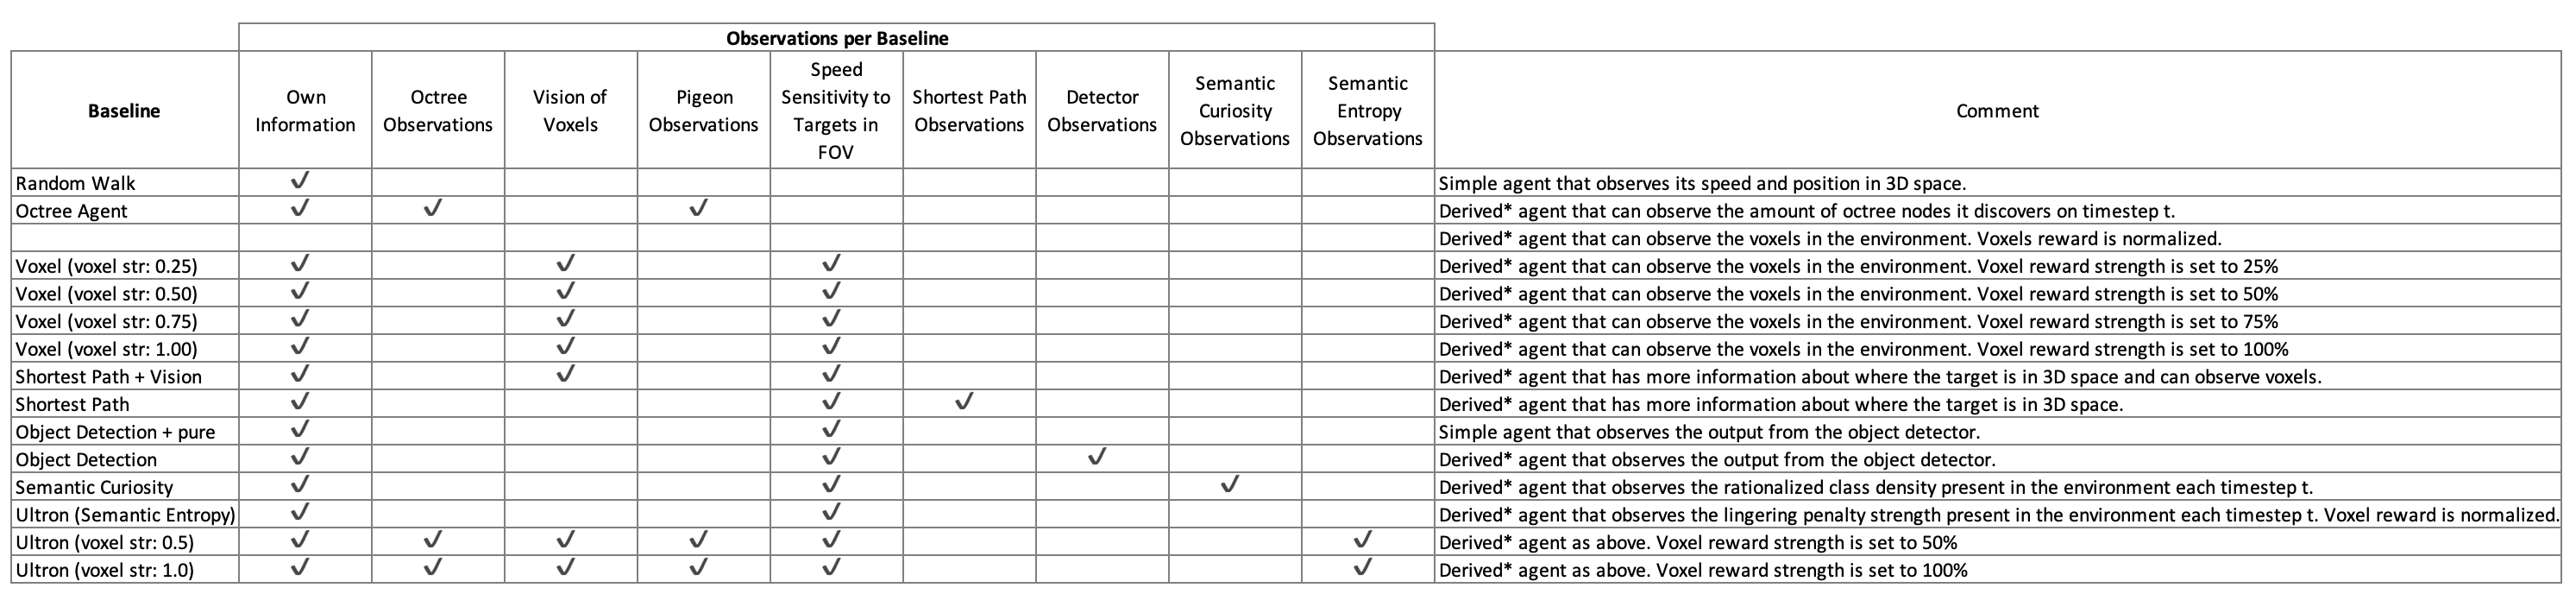
\includegraphics[width=1.5\textwidth]{images/baselines_table1.png}
%     \caption{Sample 3D assets for scenario proposals. Taken from \cite{unity-asset-store}.}
%     \label{fig:baselines_table1}
%     \end{figure}
    
%     % \begin{table}[]
%     %     \centering
%     %     \resizebox{2\textwidth}{!} {
%     %     \begin{tabular}{ | l | l | l | l | l | l | l | l | l | l | l | }
%     %     \hline
%     %     	Observations per Baseline &  &  &  &  &  &  &  &  & \  & \  \\ \hline
%     %     	Baseline & \thead{Own Information} & Octree Observations & Vision of Voxels & Pigeon Observations & Speed Sensitivity to Targets in FOV & Shortest Path Observations & Detector Observations & Semantic Curiosity Observations & Semantic Entropy Observations & Comment \\ \hline
%     %     	Random Walk & ✔️ &  &  &  &  &  &  &  &  & Simple agent that observes its speed and position in 3D space. \\ \hline
%     %     	Octree Agent & ✔️ & ✔️ &  & ✔️ &  &  &  &  &  & Derived* agent that can observe the amount of octree nodes it discovers on timestep t. \\ \hline
%     %     	 &  &  &  &  &  &  &  &  &  & Derived* agent that can observe the voxels in the environment. Voxels reward is normalized. \\ \hline
%     %     	Voxel (voxel str: 0.25) & ✔️ &  & ✔️ &  & ✔️ &  &  &  &  & Derived* agent that can observe the voxels in the environment. Voxel reward strength is set to 25\% \\ \hline
%     %     	Voxel (voxel str: 0.50) & ✔️ &  & ✔️ &  & ✔️ &  &  &  &  & Derived* agent that can observe the voxels in the environment. Voxel reward strength is set to 50\% \\ \hline
%     %     	Voxel (voxel str: 0.75) & ✔️ &  & ✔️ &  & ✔️ &  &  &  &  & Derived* agent that can observe the voxels in the environment. Voxel reward strength is set to 75\% \\ \hline
%     %     	Voxel (voxel str: 1.00) & ✔️ &  & ✔️ &  & ✔️ &  &  &  &  & Derived* agent that can observe the voxels in the environment. Voxel reward strength is set to 100\% \\ \hline
%     %     	Shortest Path + Vision & ✔️ &  & ✔️ &  & ✔️ &  &  &  &  & Derived* agent that has more information about where the target is in 3D space and can observe voxels.  \\ \hline
%     %     	Shortest Path & ✔️ &  &  &  & ✔️ & ✔️ &  &  &  & Derived* agent that has more information about where the target is in 3D space. \\ \hline
%     %     	Object Detection + pure & ✔️ &  &  &  & ✔️ &  &  &  &  & Simple agent that observes the output from the object detector. \\ \hline
%     %     	Object Detection & ✔️ &  &  &  & ✔️ &  & ✔️ &  &  & Derived* agent that observes the output from the object detector. \\ \hline
%     %     	Semantic Curiosity & ✔️ &  &  &  & ✔️ &  &  & ✔️ &  & Derived* agent that observes the rationalized class density present in the environment each timestep t. \\ \hline
%     %     	Ultron (Semantic Entropy) & ✔️ &  &  &  & ✔️ &  &  &  &  & Derived* agent that observes the lingering penalty strength present in the environment each timestep t. Voxel reward is normalized. \\ \hline
%     %     	Ultron (voxel str: 0.5) & ✔️ & ✔️ & ✔️ & ✔️ & ✔️ &  &  &  & ✔️ & Derived* agent as above. Voxel reward strength is set to 50\% \\ \hline
%     %     	Ultron (voxel str: 1.0) & ✔️ & ✔️ & ✔️ & ✔️ & ✔️ &  &  &  & ✔️ & Derived* agent as above. Voxel reward strength is set to 100\% \\ \hline
%     %     	 &  &  &  &  &  &  &  &  & \  & \  \\ \hline
%     %     	\  & \  & \  & \  & \  & \  & \  & \  & \  & \  & \  \\ \hline
%     %     	 &  &  &  &  &  &  &  &  & \  & \  \\ \hline
%     %     	 &  &  &  &  &  &  &  &  & \  & \  \\ \hline
%     %     	 &  &  &  &  &  &  &  &  & \  & \  \\ \hline
%     %     \end{tabular}
%     % }
%     %     \caption{Caption}
%     %     \label{tab:my_label}
%     % \end{table}
